\documentclass[12pt]{report}
\usepackage[utf8]{inputenc}
\usepackage[english, russian]{babel}
\usepackage{listings}
\usepackage{graphicx}
\usepackage{float}
\graphicspath{{imgs/}}
\usepackage{amsmath,amsfonts,amssymb,amsthm,mathtools} 
\usepackage{pgfplots}
\usepackage{filecontents}
\usepackage{indentfirst}
\usepackage{eucal}
\usepackage{enumitem}
\frenchspacing

\usepackage{indentfirst} % Красная строка

\usetikzlibrary{datavisualization}
\usetikzlibrary{datavisualization.formats.functions}

\usepackage{amsmath}
\usepackage{fixltx2e}
\usepackage{caption}


\definecolor{bluekeywords}{rgb}{0,0,1}
\definecolor{greencomments}{rgb}{0,0.5,0}
\definecolor{redstrings}{rgb}{0.64,0.08,0.08}
\definecolor{xmlcomments}{rgb}{0.5,0.5,0.5}
\definecolor{types}{rgb}{0.17,0.57,0.68}

\usepackage{listings}
\lstset{language=[Sharp]C,
	captionpos=t,
	numbers=left, %Nummerierung
	numberstyle=\small, % kleine Zeilennummern
	frame=single, % Oberhalb und unterhalb des Listings ist eine Linie
	stepnumber=1,                   
	numbersep=5pt,                
	showspaces=false,
	tabsize=2,
	showtabs=false,
	breaklines=true,
	showstringspaces=false,
	breakatwhitespace=true,
	escapeinside={(*@}{@*)},
	commentstyle=\color{greencomments},
	morekeywords={partial, var, value, get, set},
	keywordstyle=\color{bluekeywords},
	stringstyle=\color{redstrings},
	basicstyle=\ttfamily\small,
}

\usepackage[left=1cm,right=1cm, top=1cm,bottom=2cm,bindingoffset=0cm]{geometry}
% Для измененных титулов глав:
\usepackage{titlesec, blindtext, color} % подключаем нужные пакеты
\definecolor{gray75}{gray}{0.75} % определяем цвет
\newcommand{\hsp}{\hspace{20pt}} % длина линии в 20pt
% titleformat определяет стиль
\titleformat{\chapter}[hang]{\Huge\bfseries}{\thechapter\hsp\textcolor{gray75}{|}\hsp}{0pt}{\Huge\bfseries}

\usepackage{array}
\newcommand{\head}[2]{\multicolumn{1}{>{\centering\arraybackslash}p{#1}}{#2}}

% plot
\usepackage{pgfplots}
\usepackage{filecontents}
\usetikzlibrary{datavisualization}
\usetikzlibrary{datavisualization.formats.functions}

\begin{document}
	%\def\chaptername{} % убирает "Глава"
	\thispagestyle{empty}
	\begin{titlepage}
		\noindent \begin{minipage}{0.15\textwidth}
			
\includegraphics[width=\linewidth]{b_logo}
		\end{minipage}
		\noindent\begin{minipage}{0.9\textwidth}\centering
			\textbf{Министерство науки и высшего образования Российской Федерации}\\
			\textbf{Федеральное государственное бюджетное образовательное учреждение высшего образования}\\
			\textbf{~~~«Московский государственный технический университет имени Н.Э.~Баумана}\\
			\textbf{(национальный исследовательский университет)»}\\
			\textbf{(МГТУ им. Н.Э.~Баумана)}
		\end{minipage}
		
		\noindent\rule{18cm}{3pt}
		\newline\newline
		\noindent ФАКУЛЬТЕТ $\underline{~~~~~~~~~~~~~~~~~~~~~~~~~~~~~~~\text{«Информатика и системы управления»}~~~~~~~~~~~~~~~~~~~~~~~~~~~~~~~~~~~~~}$ \newline\newline
		\noindent КАФЕДРА $\underline{~~~~~~~~~~~~~\text{«Программное обеспечение ЭВМ и информационные технологии»}~~~~~~~~~~~~~~~~~~~~~~~}$\newline\newline\newline\newline\newline\newline\newline\newline\newline\newline\newline
		
		
		\begin{center}
			\noindent\begin{minipage}{1.3\textwidth}\centering
				\Large\textbf{  Отчет по лабораторной работе №3}\newline
				\textbf{по дисциплине \newline "Моделирование"}\newline\newline
			\end{minipage}
		\end{center}
		
		\noindent\textbf{Тема} $\underline{\text{Генерация случайных чисел}}$\newline\newline
		\noindent\textbf{Студент} $\underline{\text{Малышев И. А.}}$\newline\newline
		\noindent\textbf{Группа} $\underline{\text{ИУ7-71Б}}$\newline\newline
		\noindent\textbf{Оценка (баллы)} $\underline{\text{~~~~~~~~~~~~~~~~~~~~~~~~~~~}}$\newline\newline
		\noindent\textbf{Преподаватель: } $\underline{\text{Рудаков И. В.}}$\newline\newline\newline
		
		\begin{center}
			\vfill
			Москва~---~\the\year
			~г.
		\end{center}
	\end{titlepage}
	
	
	\setcounter{page}{2}

\chapter{Задание}
Написать программу, которая генерирует псевдослучайную последовательность одноразрядных, двухразрядных и трёхразрядных целых чисел с использование табличного и алгоритмического способа.

Для каждой сгенерированной последовательности чисел вычислить собственный количественный критерий оценки случайности.

Предусмотреть ввод десяти чисел для проверки работы программы.


\chapter{Решение}
\section{Теоретическая часть}

Среди способов получения последовательности случайных чисел различают табличный и алгоритмический.

\subsection*{Табличный способ}

Табличные генераторы случайных чисел в качестве источника случайных чисел используют специальным образом составленные таблицы, содержащие проверенные некоррелированные, то есть никак не зависящие друг от друга, цифры. Так как цифры в таблице не зависят друг от друга, то таблицу можно обходить разными способами, например, сверху вниз, или справа налево, или, скажем, можно выбирать цифры, находящиеся на четных позициях.

Достоинство данного метода в том, что он дает действительно случайные числа, так как таблица содержит проверенные некоррелированные цифры. Недостатки метода: для хранения большого количества цифр требуется много памяти; большие трудности порождения и проверки такого рода таблиц, повторы при использовании таблицы уже не гарантируют случайности числовой последовательности, а значит, и надежности результата.

\subsection*{Алгоритмический способ}

Числа, генерируемые с помощью этого способа, всегда являются псевдослучайными (или квазислучайными), то есть каждое последующее сгенерированное число зависит от предыдущего:

\begin{equation}
	r_{i+1} = f(r_i)
\end{equation}

Последовательности, составленные из таких чисел, образуют петли, то есть обязательно существует цикл, повторяющийся бесконечное число раз. Повторяющиеся циклы называются \textbf{периодами}.

Достоинством данного способа является быстродействие: генераторы практически не требуют ресурсов памяти, компактны. Недостатки: числа нельзя в полной мере назвать случайными, поскольку между ними имеется зависимость, а также наличие периодов в последовательности квазислучайных чисел.

\subsubsection*{Выбранный алгоритмический способ}

В качестве используемого метода генерации последовательности случайных чисел был выбран линейный конгруэнтный метод.
Суть данного метода заключается в вычислении последовательности случайных чисел, полагая:

\begin{equation}
	X_{n+1} = (aX_n + c) \mod m,
\end{equation}

где $X_{n+1}$ – это следующее число в последовательности, $a$ – множитель, причём $0 \leq a < m$, $c$ – приращение, причём $0 \leq c \leq m$ , $m$ – натуральное число, относительно которого вычисляется остаток от деления, причём $m \geq 2$.

При выборе значения m необходимо учитывать следующие условия:
\begin{itemize}
	\item Данное число должно быть довольно большим, так как период не может иметь более m элементов;
	\item Данное значение должно быть таким, чтобы случайные значения вычислялись быстро.
\end{itemize}

Для улучшения статистических свойств числовой последовательности во многих генераторах используется только часть битов результата.
В качестве констант в данной работе используются следующие значения:

\begin{itemize}
	\item $a=1103515245$
	\item $с=12345$
	\item $m=2^{32}$
\end{itemize}


\subsection*{Критерий оценки случайности}

В качестве критерия было предложено следующее: пусть имеется последовательность $a_i$. Берется разность между элементами последовательности $a_{i+1} - a_i$, которая образует последовательность элементов $s_i$. Если средняя вероятность появления элемента последовательности чисел $s_i$ примерно равна $\frac{1}{n}$, где $n$ -- число элементов последовательности $s_i$, то такая последовательность является случайной.

\section{Листинг}

Далее представлен фрагмент программы, выполняющий поставленное задание.

\begin{lstlisting}
internal class LCGenerator
{
	int curElem = 1;
	int a, c, m;
	
	public LCGenerator(int a, int c, int m) 
	{
		this.a = a;
		this.c = c;
		this.m = m;
	}
	
	public int Seed
	{
		get => curElem;
		set => curElem = value;
	}
	
	public IEnumerable<int> GetRandomSequence(int count, int requiredDigits)
	{
		List<int> res = new List<int>();
		
		int requiredDigitsDivider = (int)Math.Pow(10, requiredDigits);
		int minAppendValue = requiredDigitsDivider / 10 - 1;
		int addedElements = 0;
		
		for (int i = 0; i < count; i++)
		{
			curElem = (curElem * a + c) % m;
			
			if (curElem % requiredDigitsDivider >= minAppendValue)
				res.Add(curElem);
			else
				addedElements--;
		}
		
		return res;
	}
}

internal static class Criteria
{
	public static double TestCriteria(IEnumerable<int> sequence)
	{
		List<int> s = new List<int>();
		
		for (int i = 0; i < sequence.Count() - 1; i++) 
		{
			var elem = sequence.ElementAt(i + 1) - sequence.ElementAt(i);
			
			if (!s.Contains(elem))
				s.Add(elem);
		}
		
		int sCount = s.Count();
		
		int[] references = new int[sCount];
		
		for (int i = 0; i < sCount; i++)
			for (int j = 0; j < sCount; j++)
			{
				if (i != j && s[i] == s[j])
					references[i]++;
			}
		
		return references.Select(x => x / (double)sCount).Sum() / sCount;
	}
}
\end{lstlisting}

\section{Результаты работы}

На рисунках \ref{img:ui1}-\ref{img:ui2} представлен пользовательский интерфейс программы до ввода количества состояний и ввода интенсивностей.

\begin{figure}[H]
	\begin{center}
		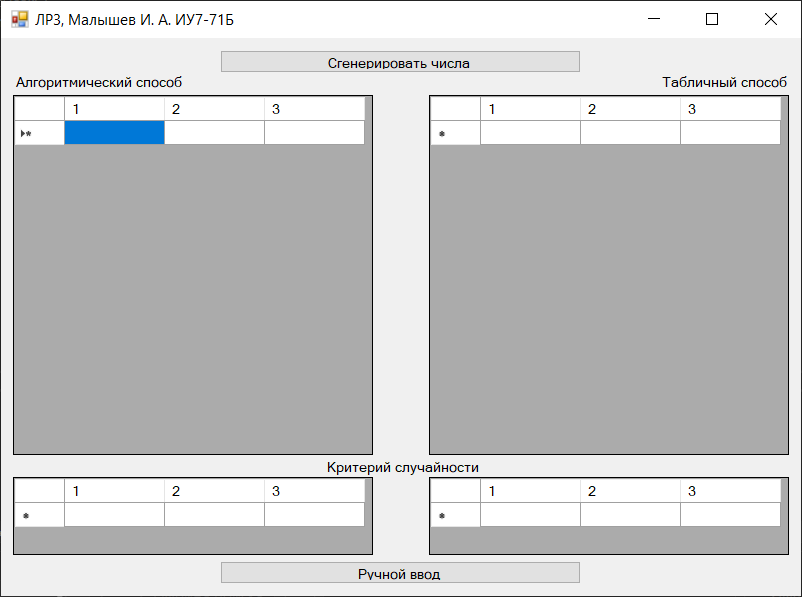
\includegraphics[scale=0.6]{imgs/ui1.png}
	\end{center}
	\caption{Пользовательский интерфейс программы до ввода количества состояний.}
	\label{img:ui1}
\end{figure}

\begin{figure}[H]
	\begin{center}
		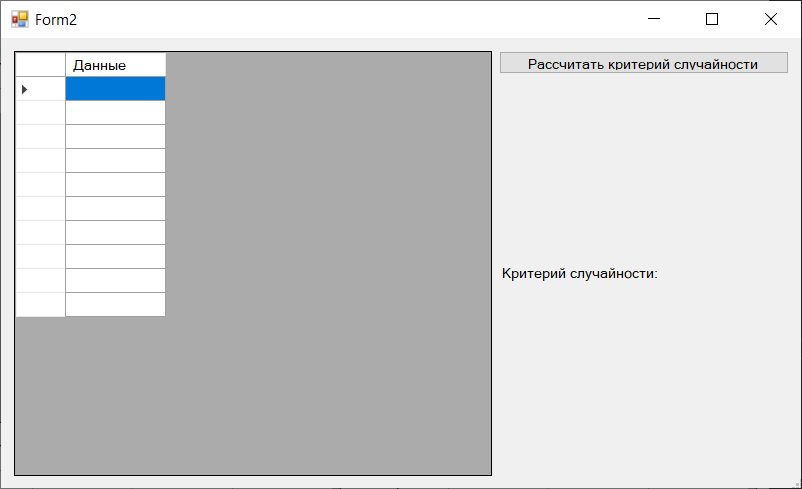
\includegraphics[scale=0.6]{imgs/ui2.png}
	\end{center}
	\caption{Пользовательский интерфейс программы до ввода интенсивностей.}
	\label{img:ui2}
\end{figure}

\subsection{Пример 1}

На рисунках \ref{img:res2}-\ref{img:graph2} представлен пример результатов работы программы с указанными данными.

\begin{figure}[H]
	\begin{center}
		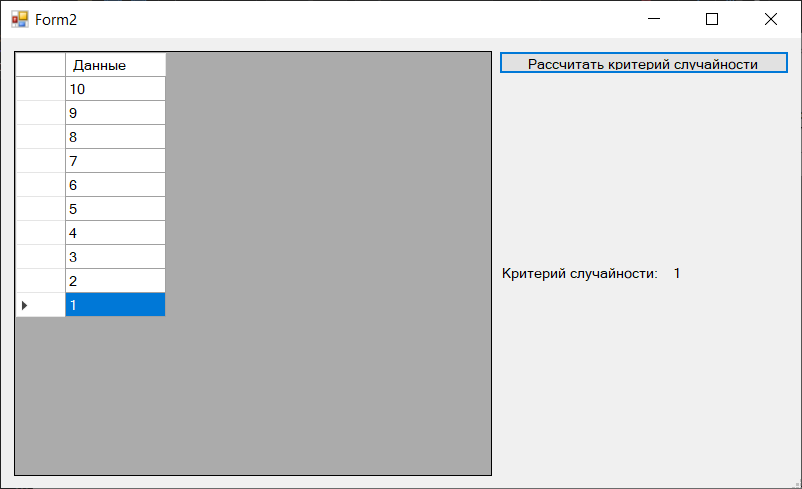
\includegraphics[scale=0.6]{imgs/res2.png}
	\end{center}
	\caption{Исходные данные и результат.}
	\label{img:res2}
\end{figure}

\begin{figure}[H]
	\begin{center}
		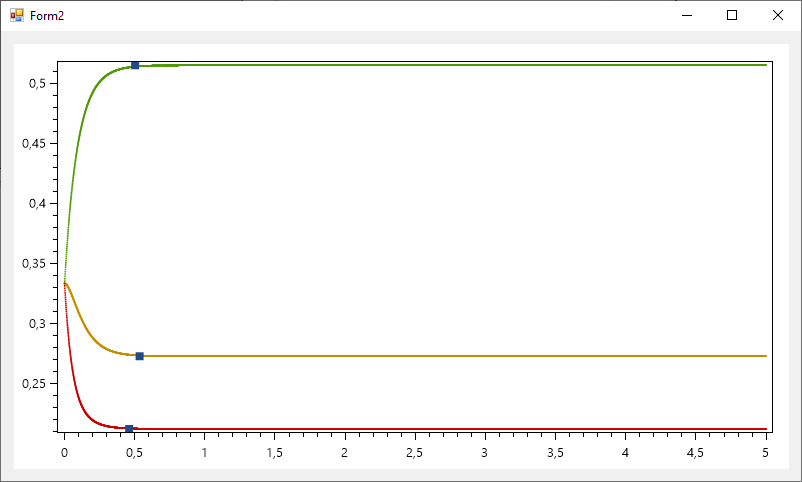
\includegraphics[scale=0.6]{imgs/graph2.png}
	\end{center}
	\caption{График вероятностей с точками стабилизации.}
	\label{img:graph2}
\end{figure}

\subsection{Пример 2}

На рисунках \ref{img:res1}-\ref{img:graph1} представлен пример результатов работы программы с указанными данными.

\begin{figure}[H]
	\begin{center}
		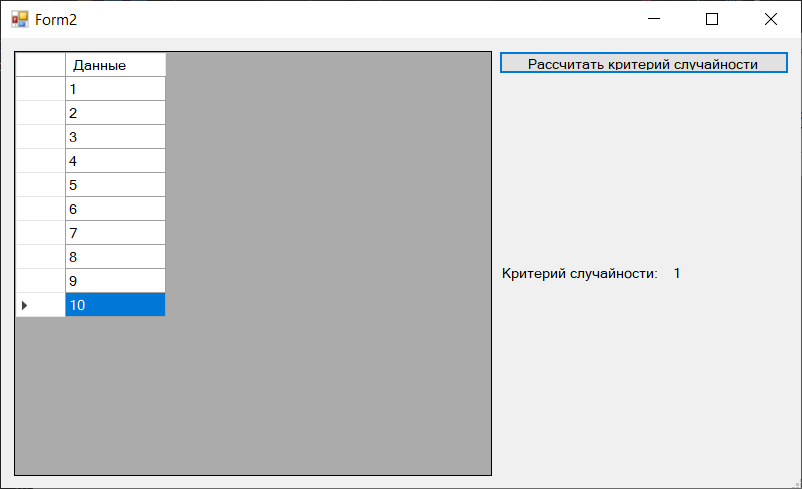
\includegraphics[scale=0.6]{imgs/res1.png}
	\end{center}
	\caption{Исходные данные и результат.}
	\label{img:res1}
\end{figure}

\begin{figure}[H]
	\begin{center}
		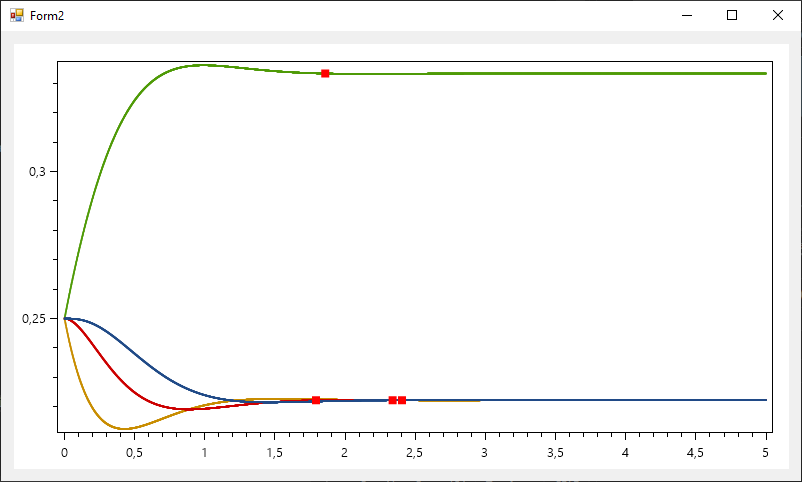
\includegraphics[scale=0.6]{imgs/graph1.png}
	\end{center}
	\caption{График вероятностей с точками стабилизации.}
	\label{img:graph1}
\end{figure}

\end{document}